%\documentclass[11pt]{paper}
%\usepackage{fullpage}
%\usepackage{palatino}
%\usepackage{amsfonts,amsmath,amssymb}
%% \usepackage{graphicx}
%
%\usepackage{listings}
%\usepackage{textcomp}
%\usepackage{color}
%
%\definecolor{dkgreen}{rgb}{0,0.6,0}
%\definecolor{gray}{rgb}{0.5,0.5,0.5}
%\definecolor{mauve}{rgb}{0.58,0,0.82}
%
%\lstset{frame=tb,
%  language=R,
%  aboveskip=3mm,
%  belowskip=3mm,
%  showstringspaces=false,
%  columns=flexible,
%  basicstyle={\small\ttfamily},
%  numbers=none,
%  numberstyle=\tiny\color{gray},
%  keywordstyle=\color{blue},
%  commentstyle=\color{dkgreen},
%  stringstyle=\color{mauve},
%  breaklines=true,
%  breakatwhitespace=true,
%  tabsize=3
%}
%
%
%
%\ifx\pdftexversion\undefined
%    \usepackage[dvips]{graphicx}
%\else
%    \usepackage[pdftex]{graphicx}
%    \usepackage{epstopdf}
%    \epstopdfsetup{suffix=}
%\fi
%
%\usepackage{subfig}
%
%
%
%% Trying different tips from Google help to get a summary to print.
%% \usepackage[T1]{fontenc} 
%% \usepackage[utf8]{inputenc}
%% 
%% \usepackage[utf8]{inputenc}
%% \usepackage[utf8x]{inputenc}
%\UseRawInputEncoding
%% This allows pdflatex to print the curly quotes in the
%% significance codes in the output of the GAM.
%
%
%\begin{document}

%%%%%%%%%%%%%%%%%%%%%%%%%%%%%%%%%%%%%%%%
% Problem Set 7
%%%%%%%%%%%%%%%%%%%%%%%%%%%%%%%%%%%%%%%%

%\pagestyle{empty}
%{\noindent\bf Spring 2021 \hfill Firstname M.~Lastname}
%\vskip 16pt
%\centerline{\bf University of Central Florida}
%\centerline{\bf College of Business}
%\vskip 16pt
%\centerline{\bf QMB 6911}
%\centerline{\bf Capstone Project in Business Analytics}
%\vskip 10pt
%\centerline{\bf Solutions:  Problem Set \#8}
%\vskip 32pt
%\noindent
%% 
%% 
%\section{Data Description}
%% 
%By engaging an industry consultant to gather relevant and appropriate 
%information, your firm has been able to put together data concerning 248 
%different fly-fishing reels, over one-half of which are produced in the 
%United States, with the remainder being produced in Asia---either in China 
%or Korea.  These data are contained in the file {\tt FlyReels.csv}, which is
%available in the {\tt Data} folder.
%Each fly-fishing reel in the data set is a row, while the columns correspond 
%to the variables whose names and definitions are the following:
%\bigskip
%\begin{table}[ht]
%\centering
%\begin{tabular}{ll}
%  \hline
%    Variable & Definition \\
%  \hline
%
%    {\tt Name}        &product name (a string) \\ 
%    {\tt Brand}       &brand name (a string) \\ 
%    {\tt Weight}      &weight of reel in ounces (a real number) \\ 
%    {\tt Diameter}    &diameter of reel in inches (a real number) \\ 
%    {\tt Width}       &width of reel in inches (a real number) \\ 
%    {\tt Price}       &price of reel in dollars (a real number) \\ 
%    {\tt Sealed}      &whether the reel is sealed; {\tt "Yes"} versus
%                        {\tt "No"} (a string) \\ 
%    {\tt Country}     &country of manufacture, (a string) \\ 
%    {\tt Machined}    &whether the reel is machined versus cast;
%                        machined={\tt "Yes"}, \\ 
%                      &while cast={\tt "No"} (a string) \\ 
%  \hline
%\end{tabular}
%%\caption{Summary of Numeric Variables}
%%\label{tab:summary}
%\end{table}


I will revisit the recommended linear model
from Problem Set \#7, 
which included 



I will investigate any nonlinear relationships
by incorporating a nonparametric specification
for the value of the dimensions of the reels:
the width, diameter, and density, 
which constitute the continuous variables in the dataset.
The nonparametric analysis will be performed
to investigate whether the value of these characteristics
are best described with nonlinear forms. 


%%%%%%%%%%%%%%%%%%%%%%%%%%%%%%%%%%%%%%%%
\clearpage
\section{Linear Regression Model}
%%%%%%%%%%%%%%%%%%%%%%%%%%%%%%%%%%%%%%%%

A natural staring point is the recommended linear model
from Problem Set \#7. 

\subsection{Linear Model with \texttt{Sealed*Made\_in\_USA} Interaction}

Last week I investigated whether 
the functional form should include different specifications by
country of manufacture.
% 
The model included the continuous variables 
width, diameter, and density, 
as well as categorical variables for 
country of manufacture, 
and whether or not the reels were sealed or machined. 
% 
In addition to the indicator for the country of manufacture, the model included an indicator for an interaction between
the the country of manufacture indicator and the indicator for whether the reels were sealed or unsealed. 
% 
The dependent variable was chosen as 
the logarithm of the fly reel price, 
since the results were similar to those from the model 
with the optimal Box-Cox transformation, 
without the added complexity. 
% 
The results of this regression specification are shown in 
Table \ref{tab:reg_sealed_USA}. 
% 

\begin{table}
\begin{center}
\begin{tabular}{l c}
\hline
 & Model 1 \\
\hline
(Intercept)                 & $2.00999^{***}$ \\
                            & $(0.26125)$     \\
Width                       & $0.33575^{*}$   \\
                            & $(0.15622)$     \\
Diameter                    & $0.39567^{***}$ \\
                            & $(0.05076)$     \\
Density                     & $1.21296^{***}$ \\
                            & $(0.21948)$     \\
SealedYes                   & $0.62731^{***}$ \\
                            & $(0.08622)$     \\
MachinedYes                 & $0.64934^{***}$ \\
                            & $(0.08320)$     \\
made\_in\_USATRUE           & $0.74633^{***}$ \\
                            & $(0.09247)$     \\
SealedYes:made\_in\_USATRUE & $-0.29519^{**}$ \\
                            & $(0.10092)$     \\
\hline
R$^2$                       & $0.74893$       \\
Adj. R$^2$                  & $0.74160$       \\
Num. obs.                   & $248$           \\
\hline
\multicolumn{2}{l}{\scriptsize{$^{***}p<0.001$; $^{**}p<0.01$; $^{*}p<0.05$}}
\end{tabular}
\caption{Linear Model for Fly Reel Prices}
\label{tab:reg_sealed_USA}
\end{center}
\end{table}

% 
Next, I will attempt to improve on this specification
by investigating the potential for nonlinear functional forms. 







%%%%%%%%%%%%%%%%%%%%%%%%%%%%%%%%%%%%%%%%
\clearpage
\section{Nonlinear Specifications}
%%%%%%%%%%%%%%%%%%%%%%%%%%%%%%%%%%%%%%%%


% \clearpage
\subsection{Nonparametric Specification for Width}

As above, I first conduct FWL regressions 
to reduce the problem to two dimensions. 
The results are not shown here, 
since the comparison only verifies 
the conclusion of the FWL theorem. 

To illustrate the fit of the linear model, 
Figure \ref{fig:dev_vs_width} shows a scatter plot 
of the residual log prices on 
the width of fly reels. 
The observations are shown in blue
and the fitted values are shown in red.
The variation in the fitted values results from the 
fact that it is not plotted against the transformed 
excess width variable 
used in the regressions.
Still, the linear pattern is apparent
and appears to match the data. 

\begin{figure}[h!]
  \centering
  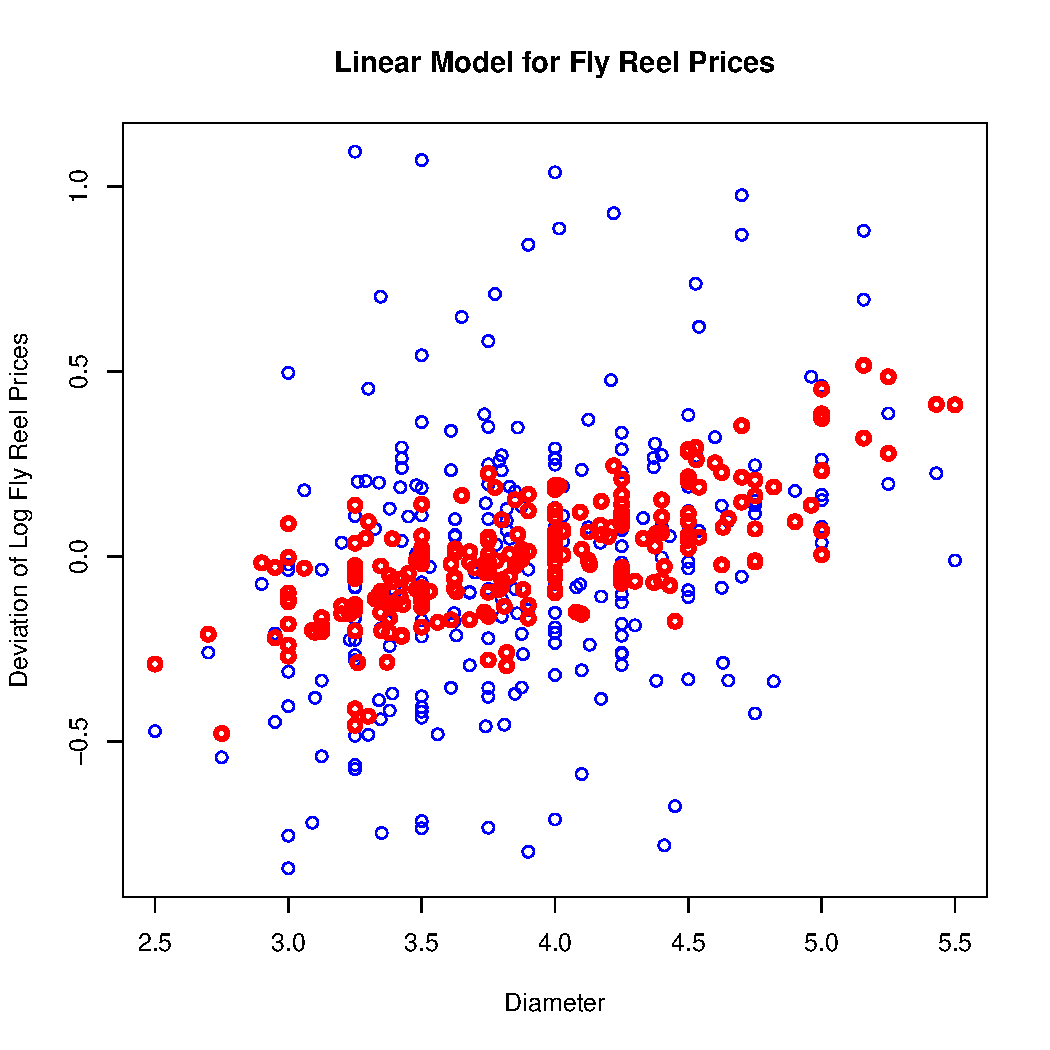
\includegraphics[scale = 0.5, keepaspectratio=true]{../Figures/dev_vs_diameter}
  \caption{Linear Model for Fly Reel Prices vs. Width} \label{fig:dev_vs_width}
\end{figure}



\pagebreak
As a comparison, Figure \ref{fig:dev_np_vs_width_dev} 
augments the above by showing the plot against the 
residuals from the regression for 
width:
the ``excess width'' of a fly reel 
compared to what would be 
expected given the other characteristics of the fly reel. 
The fit follows a straight line, as specified in the model. 
% 
I move directly to the nonparametric specification for 
the relationship between prices and 
width.
Figure \ref{fig:dev_np_vs_width_dev} 
overlays the nonparametric estimate, shown in green. 
The pattern has more variation in slope but 
closely follows the prediction from the linear model. 
Although the nonparametric estimate varies around the linear estimate,
it appears that the linear form
is also a close enough approximation.


\begin{figure}[h!]
  \centering
  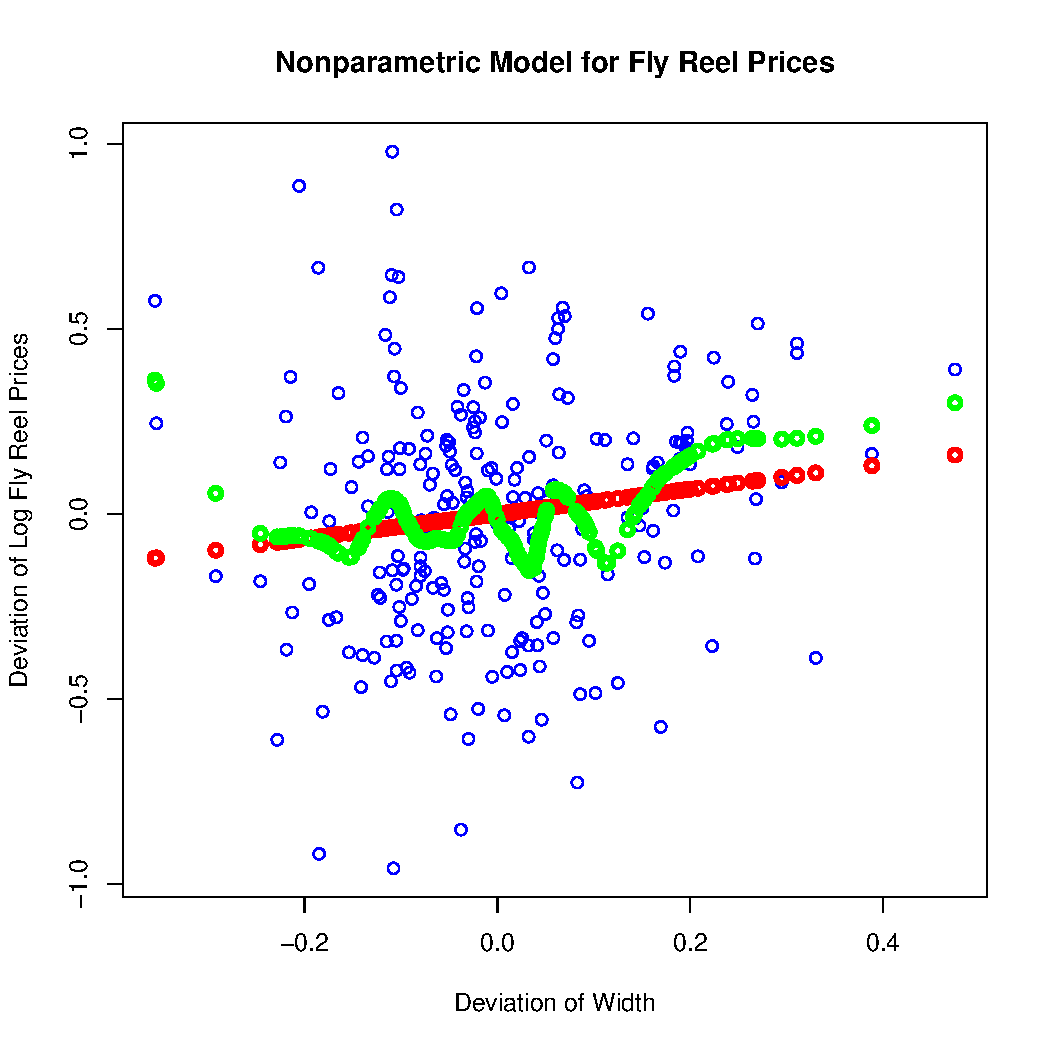
\includegraphics[scale = 0.5, keepaspectratio=true]{../Figures/dev_np_vs_width_dev}
  \caption{Nonparametric Model for Fly Reel Prices: Excess Width} \label{fig:dev_np_vs_width_dev}
\end{figure}


\clearpage
\subsection{Nonparametric Specification for Diameter}

To illustrate the fit of the linear model, 
Figure \ref{fig:dev_vs_diameter} shows a scatter plot 
of the residual log prices on 
the diameter of fly reels. 
The observations are shown in blue
and the fitted values are shown in red.
The variation in the fitted values results from the 
fact that it is not plotted against the transformed 
excess diameter variable 
used in the regressions.
Still, the linear pattern is apparent
and appears to match the data. 

\begin{figure}[h!]
  \centering
  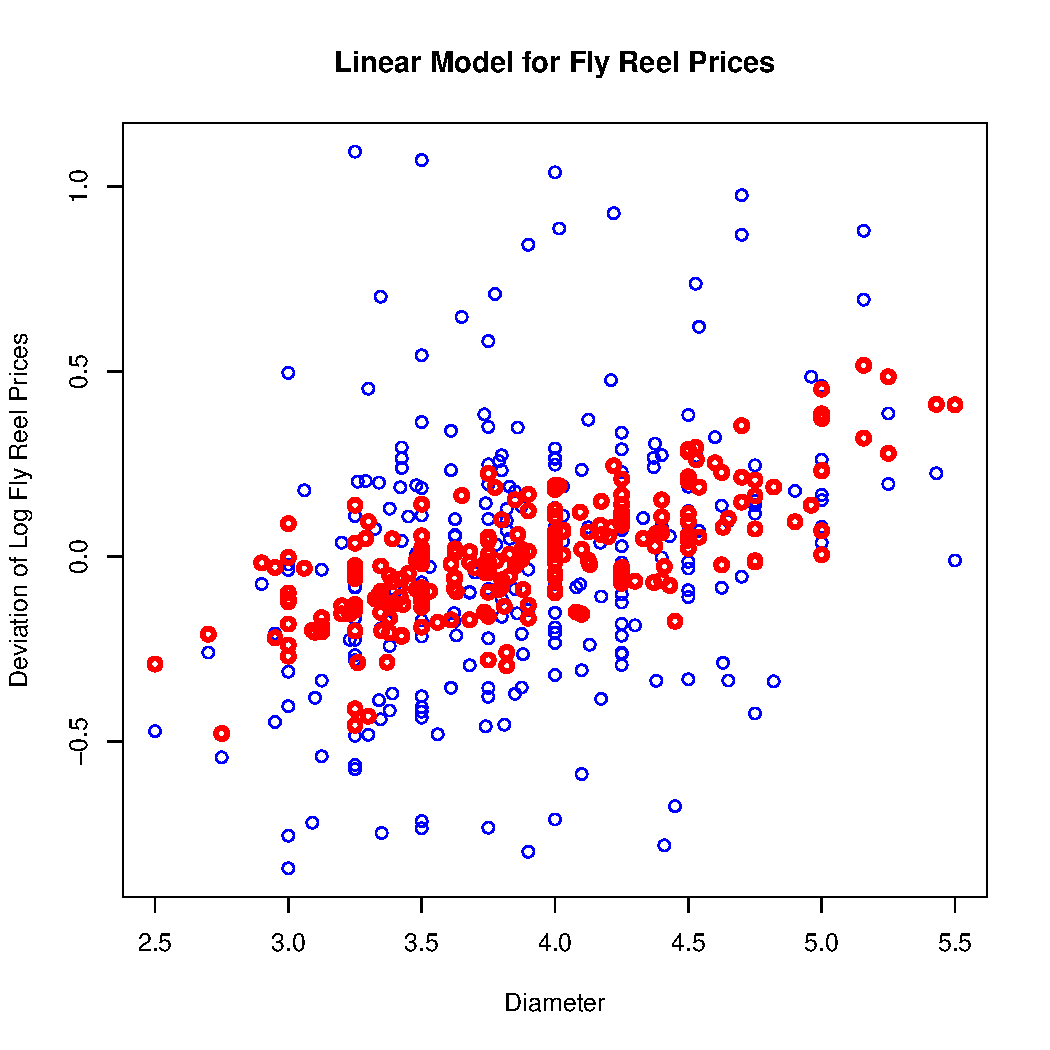
\includegraphics[scale = 0.5, keepaspectratio=true]{../Figures/dev_vs_diameter}
  \caption{Linear Model for Fly Reel Prices vs. Diameter} \label{fig:dev_vs_diameter}
\end{figure}



\pagebreak
As a comparison, Figure \ref{fig:dev_np_vs_diameter_dev} 
augments the above by showing the plot against the 
residuals from the regression for 
diameter:
the ``excess diameter'' of a fly reel 
compared to what would be 
expected given the other characteristics of the fly reel. 
The fit follows a straight line, as specified in the model. 
% 
I move directly to the nonparametric specification for 
the relationship between prices and 
diameter.
Figure \ref{fig:dev_np_vs_diameter_dev} 
overlays the nonparametric estimate, shown in green. 
The pattern has more variation in slope but 
closely follows the prediction from the linear model. 
Although the nonparametric estimate varies around the linear estimate,
it appears that the linear form
is also a close enough approximation.


\begin{figure}[h!]
  \centering
  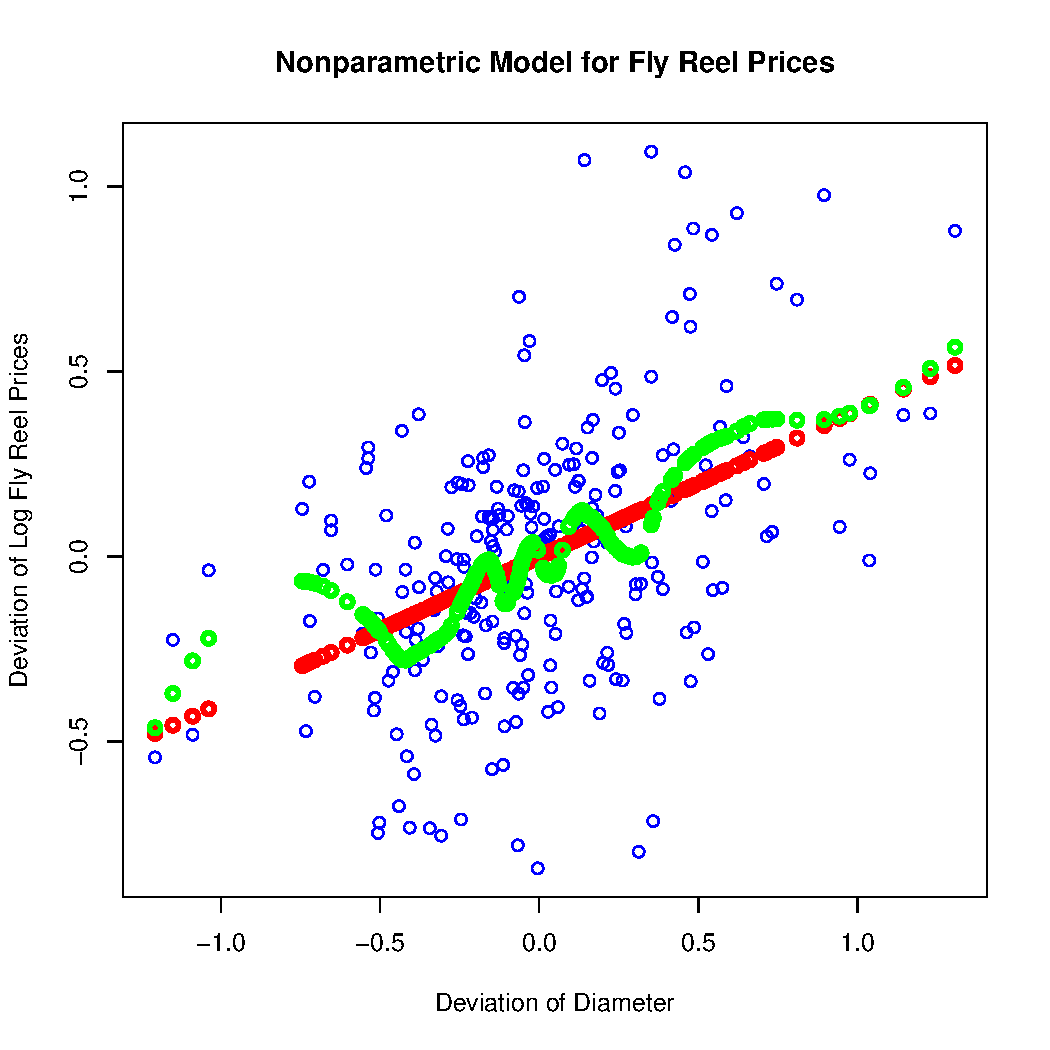
\includegraphics[scale = 0.5, keepaspectratio=true]{../Figures/dev_np_vs_diameter_dev}
  \caption{Nonparametric Model for Fly Reel Prices: Excess Diameter} \label{fig:dev_np_vs_diameter_dev}
\end{figure}



\clearpage
\subsection{Nonparametric Specification for Density}

To illustrate the fit of the linear model, 
Figure \ref{fig:dev_vs_density} shows a scatter plot 
of the residual log prices on 
the density of fly reels. 
The observations are shown in blue
and the fitted values are shown in red.
The variation in the fitted values results from the 
fact that it is not plotted against the transformed 
excess density variable 
used in the regressions.
Still, the linear pattern is apparent
and appears to match the data. 

\begin{figure}[h!]
  \centering
  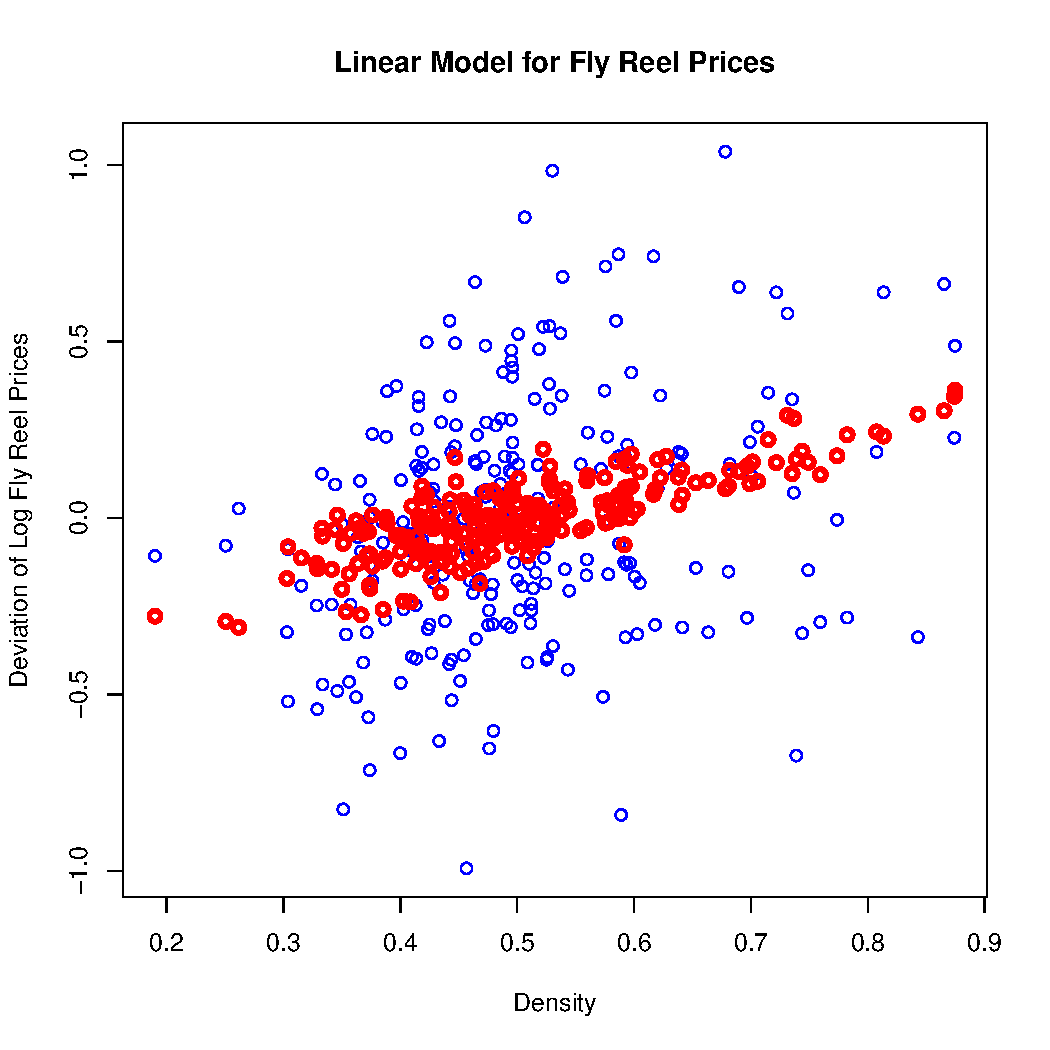
\includegraphics[scale = 0.5, keepaspectratio=true]{../Figures/dev_vs_density}
  \caption{Linear Model for Fly Reel Prices vs. Density} \label{fig:dev_vs_density}
\end{figure}



\pagebreak
As a comparison, Figure \ref{fig:dev_np_vs_density_dev} 
augments the above by showing the plot against the 
residuals from the regression for 
density:
the ``excess density'' of a fly reel 
compared to what would be 
expected given the other characteristics of the fly reel. 
The fit follows a straight line, as specified in the model. 
% 
I move directly to the nonparametric specification for 
the relationship between prices and 
density.
Figure \ref{fig:dev_np_vs_density_dev} 
overlays the nonparametric estimate, shown in green. 
The pattern has more variation in slope but 
closely follows the prediction from the linear model. 
Although the nonparametric estimate varies around the linear estimate,
it appears that the linear form
is also a close enough approximation.


\begin{figure}[h!]
  \centering
  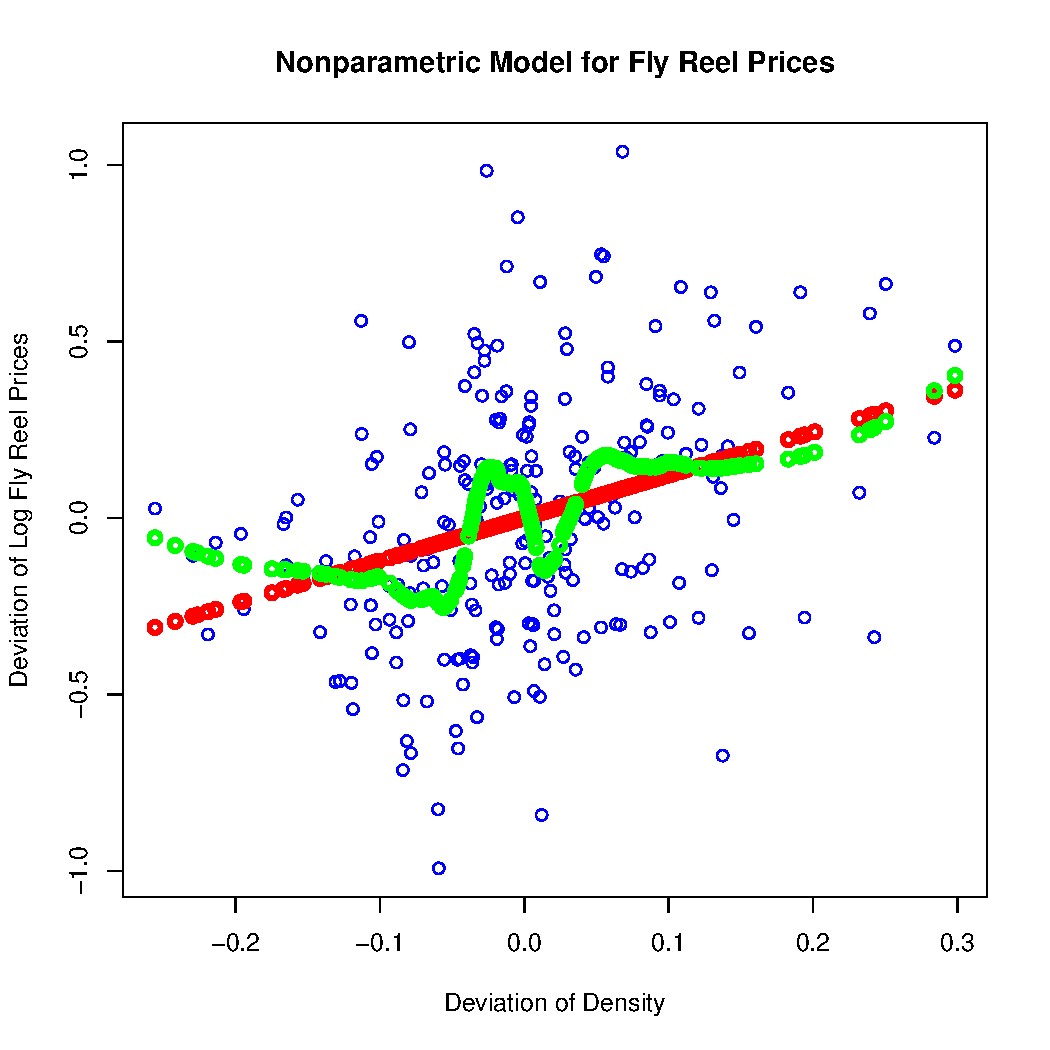
\includegraphics[scale = 0.5, keepaspectratio=true]{../Figures/dev_np_vs_density_dev}
  \caption{Nonparametric Model for Fly Reel Prices: Excess Density} \label{fig:dev_np_vs_density_dev}
\end{figure}

 

\pagebreak
\section{Semiparametric Estimates}

As I was building the above nonparametric models, 
I stored the predictions and will now use them as variables in 
linear models. 
Table \ref{tab:reg_semipar} 
shows the estimates from a set of models. 
Model 1 is the benchmark linear model in 
Table \ref{tab:reg_sealed_USA}. 
Model 2 is a semi-parametric model
with a nonparametric fit on width
substituted in for the width variable.
Models 3 and 4 are semi-parametric models
with nonparametric fits on diameter and density, respectively.
Model 5 is a maximally semiparametric model, 
with nonparametric fits for all continuous variables. 
For each of the single-variable semiparametric models, 
the coefficients are near one
and the fits are similar to the linear model. 
Even with maximal flexibility, the fit of Model 5
is slightly better than the benchmark linear model. 
Across all models, the adjusted $\bar{R}^2$ values are all hovering around 0.75, 
with the full parametric model up to 0.80. 
All things considered, these are excellent models
and the linear model is sufficient
but you might recommend the full semiparametric model
if you can justify the additional complexity.

One factor to keep in mind, however,
is that the above semiparametric models
essentially take the nonparametric functions as known, 
and do not account for the additional variability of
the nonarametric parts of the model.
The next specification estimates both linear 
and nonlinear parts jointly. 


\begin{table}
\begin{center}
\begin{tabular}{l c c c c c}
\hline
 & Model 1 & Model 2 & Model 3 & Model 4 & Model 5 \\
\hline
(Intercept)                 & $2.00999^{***}$ & $2.34926^{***}$ & $2.98091^{***}$  & $3.23438^{***}$ & $4.49531^{***}$  \\
                            & $(0.26125)$     & $(0.22596)$     & $(0.22704)$      & $(0.15261)$     & $(0.05897)$      \\
Width                       & $0.33575^{*}$   &                 & $0.92791^{***}$  & $0.03044$       &                  \\
                            & $(0.15622)$     &                 & $(0.12784)$      & $(0.14082)$     &                  \\
Diameter                    & $0.39567^{***}$ & $0.43144^{***}$ &                  & $0.33658^{***}$ &                  \\
                            & $(0.05076)$     & $(0.04150)$     &                  & $(0.04671)$     &                  \\
Density                     & $1.21296^{***}$ & $1.07566^{***}$ & $0.81613^{***}$  &                 &                  \\
                            & $(0.21948)$     & $(0.20093)$     & $(0.20645)$      &                 &                  \\
SealedYes                   & $0.62731^{***}$ & $0.61960^{***}$ & $0.70050^{***}$  & $0.56858^{***}$ & $0.69858^{***}$  \\
                            & $(0.08622)$     & $(0.08246)$     & $(0.08226)$      & $(0.08047)$     & $(0.07509)$      \\
MachinedYes                 & $0.64934^{***}$ & $0.58954^{***}$ & $0.71659^{***}$  & $0.65070^{***}$ & $0.61103^{***}$  \\
                            & $(0.08320)$     & $(0.07933)$     & $(0.07938)$      & $(0.07819)$     & $(0.07386)$      \\
made\_in\_USATRUE           & $0.74633^{***}$ & $0.77354^{***}$ & $0.79615^{***}$  & $0.70473^{***}$ & $0.79326^{***}$  \\
                            & $(0.09247)$     & $(0.08855)$     & $(0.08879)$      & $(0.08692)$     & $(0.08296)$      \\
SealedYes:made\_in\_USATRUE & $-0.29519^{**}$ & $-0.29826^{**}$ & $-0.33376^{***}$ & $-0.27253^{**}$ & $-0.31356^{***}$ \\
                            & $(0.10092)$     & $(0.09642)$     & $(0.09694)$      & $(0.09500)$     & $(0.09038)$      \\
width\_np                   &                 & $1.11995^{***}$ &                  &                 & $1.35512^{***}$  \\
                            &                 & $(0.21565)$     &                  &                 & $(0.20456)$      \\
diameter\_np                &                 &                 & $1.00650^{***}$  &                 & $1.00083^{***}$  \\
                            &                 &                 & $(0.10926)$      &                 & $(0.10411)$      \\
density\_np                 &                 &                 &                  & $1.03923^{***}$ & $0.76790^{***}$  \\
                            &                 &                 &                  & $(0.12864)$     & $(0.12582)$      \\
\hline
R$^2$                       & $0.74893$       & $0.76995$       & $0.76755$        & $0.77748$       & $0.79771$        \\
Adj. R$^2$                  & $0.74160$       & $0.76324$       & $0.76077$        & $0.77099$       & $0.79181$        \\
Num. obs.                   & $248$           & $248$           & $248$            & $248$           & $248$            \\
\hline
\multicolumn{6}{l}{\scriptsize{$^{***}p<0.001$; $^{**}p<0.01$; $^{*}p<0.05$}}
\end{tabular}
\caption{Semiparametric Models for Fly Reel Prices}
\label{tab:reg_semipar}
\end{center}
\end{table}



\pagebreak
\section{Generalized Additive Model}

\subsection{Linear Model}

As an example of the output from the GAM specification, 
I first estimated the model with no nonlinear terms, 
which is essentially a linear regression. 

\begin{verbatim}
Family: gaussian 
Link function: identity 

Formula:
log_Price ~ Width + Diameter + Density + Sealed + Machined + 
    made_in_USA + made_in_USA * Sealed

Parametric coefficients:
                          Estimate Std. Error t value Pr(>|t|)    
(Intercept)                2.00999    0.26125   7.694 3.69e-13 ***
Width                      0.33575    0.15622   2.149  0.03262 *  
Diameter                   0.39567    0.05076   7.795 1.95e-13 ***
Density                    1.21296    0.21948   5.527 8.49e-08 ***
SealedYes                  0.62731    0.08622   7.275 4.88e-12 ***
MachinedYes                0.64934    0.08320   7.805 1.84e-13 ***
made_in_USATRUE            0.74633    0.09247   8.071 3.35e-14 ***
SealedYes:made_in_USATRUE -0.29519    0.10092  -2.925  0.00378 ** 
---
Signif. codes:  0 �***� 0.001 �**� 0.01 �*� 0.05 �.� 0.1 � � 1


R-sq.(adj) =  0.742   Deviance explained = 74.9%
GCV = 0.10913  Scale est. = 0.10561   n = 248
\end{verbatim}

\pagebreak
\subsection{Semiparametric Model}


Since the results of the full semiparametric specification,
in Model 5 of Table \ref{tab:reg_semipar},
were so promising, 
I estimated the model with all three continuous variables specified as nonparametric functions. 
The result was that 
all the variables---both linear and nonlinear---were 
statistically significant. 
On the other hand, 
the adjusted R-squared has not increased very much, 
from 0.742 to 0.769 under this specification, 
which may not justify the added complexity of the model.
Perhaps more importantly, the coefficients on the 
linear terms are very similar across models, 
indicating that the models support similar conclusions relating to any business decision involving
the ``Made in USA'' premium. 
With this second model, we have even more support for those conclusions
and are certain that the conclusions are not 
coincidental results of the
functional form decisions for previous models.

\begin{verbatim}
Family: gaussian 
Link function: identity 

Formula:
log_saleprice ~ s(horsepower) + s(age) + s(enghours) + diesel + 
    fwd + manual + johndeere + cab

Parametric coefficients:
            Estimate Std. Error t value Pr(>|t|)    
(Intercept)  9.04516    0.09366  96.575  < 2e-16 ***
diesel       0.13440    0.09499   1.415  0.15830    
fwd          0.29899    0.05754   5.196 4.11e-07 ***
manual      -0.16938    0.05965  -2.839  0.00487 ** 
johndeere    0.33067    0.06890   4.799 2.68e-06 ***
cab          0.40439    0.07151   5.655 4.08e-08 ***
---
Signif. codes:  0 �***� 0.001 �**� 0.01 �*� 0.05 �.� 0.1 � � 1

Approximate significance of smooth terms:
                edf Ref.df     F  p-value    
s(horsepower) 4.387  5.321 44.89  < 2e-16 ***
s(age)        3.264  4.057 21.59  < 2e-16 ***
s(enghours)   1.000  1.000 23.39 2.64e-06 ***
---
Signif. codes:  0 �***� 0.001 �**� 0.01 �*� 0.05 �.� 0.1 � � 1

R-sq.(adj) =  0.819   Deviance explained = 82.8%
GCV = 0.15063  Scale est. = 0.14263   n = 276
\end{verbatim}
 

%%%%%%%%%%%%%%%%%%%%%%%%%%%%%%%%%%%%%%%%
% \end{document}
%%%%%%%%%%%%%%%%%%%%%%%%%%%%%%%%%%%%%%%%
